\chapter{Projects and planning}
\label{ch:projects}

\section{What will you achieve?}

The Projects app organizes work needing a plan, resources, and reviewable results. An administrator manages configuration and access, the work manager plans and monitors delivery, and employees update assigned records. Start with a plan when defining direction or outcomes, and with a project when delivering a defined scope.

\begin{rcnote}[Example: Horizon]
Sarah Al-Khatib uses a plan to improve Horizon visit readiness and tracks a project preparing the Aleppo branch visit. Omar Haddad prepares the visit pack, and Sarah reviews its deliverables before treating preparation as complete.
\end{rcnote}
\begin{figure}[H]
\centering
\begin{tikzpicture}[node distance=0.5cm]
\node[stepBox] (n0) {Define result and owner};
\node[stepBox,below=of n0] (n1) {Set up and approve work};
\node[stepBox,below=of n1] (n2) {Deliver and review};
\draw[flowsTo] (n0) -- (n1);
\draw[flowsTo] (n1) -- (n2);
\end{tikzpicture}
\rclegend
\caption{From intended result to delivery review}
\label{fig:projects-overview}
\shotnote{The diagram puts the intended result and ownership before delivery, then connects review to actual results. Creating a plan does not automatically create or approve a project; each record has its own actions and accountability.}
\end{figure}

A portfolio groups programs and projects around common priorities; a program coordinates related projects. These links are optional in a project definition, so do not create a portfolio or program merely to reach Projects. These plans and projects are distinct from the Epics tab in Tasks.

\section{Projects and planning page directory}
\label{sec:projects-pages}
\begin{figure}[H]
\centering
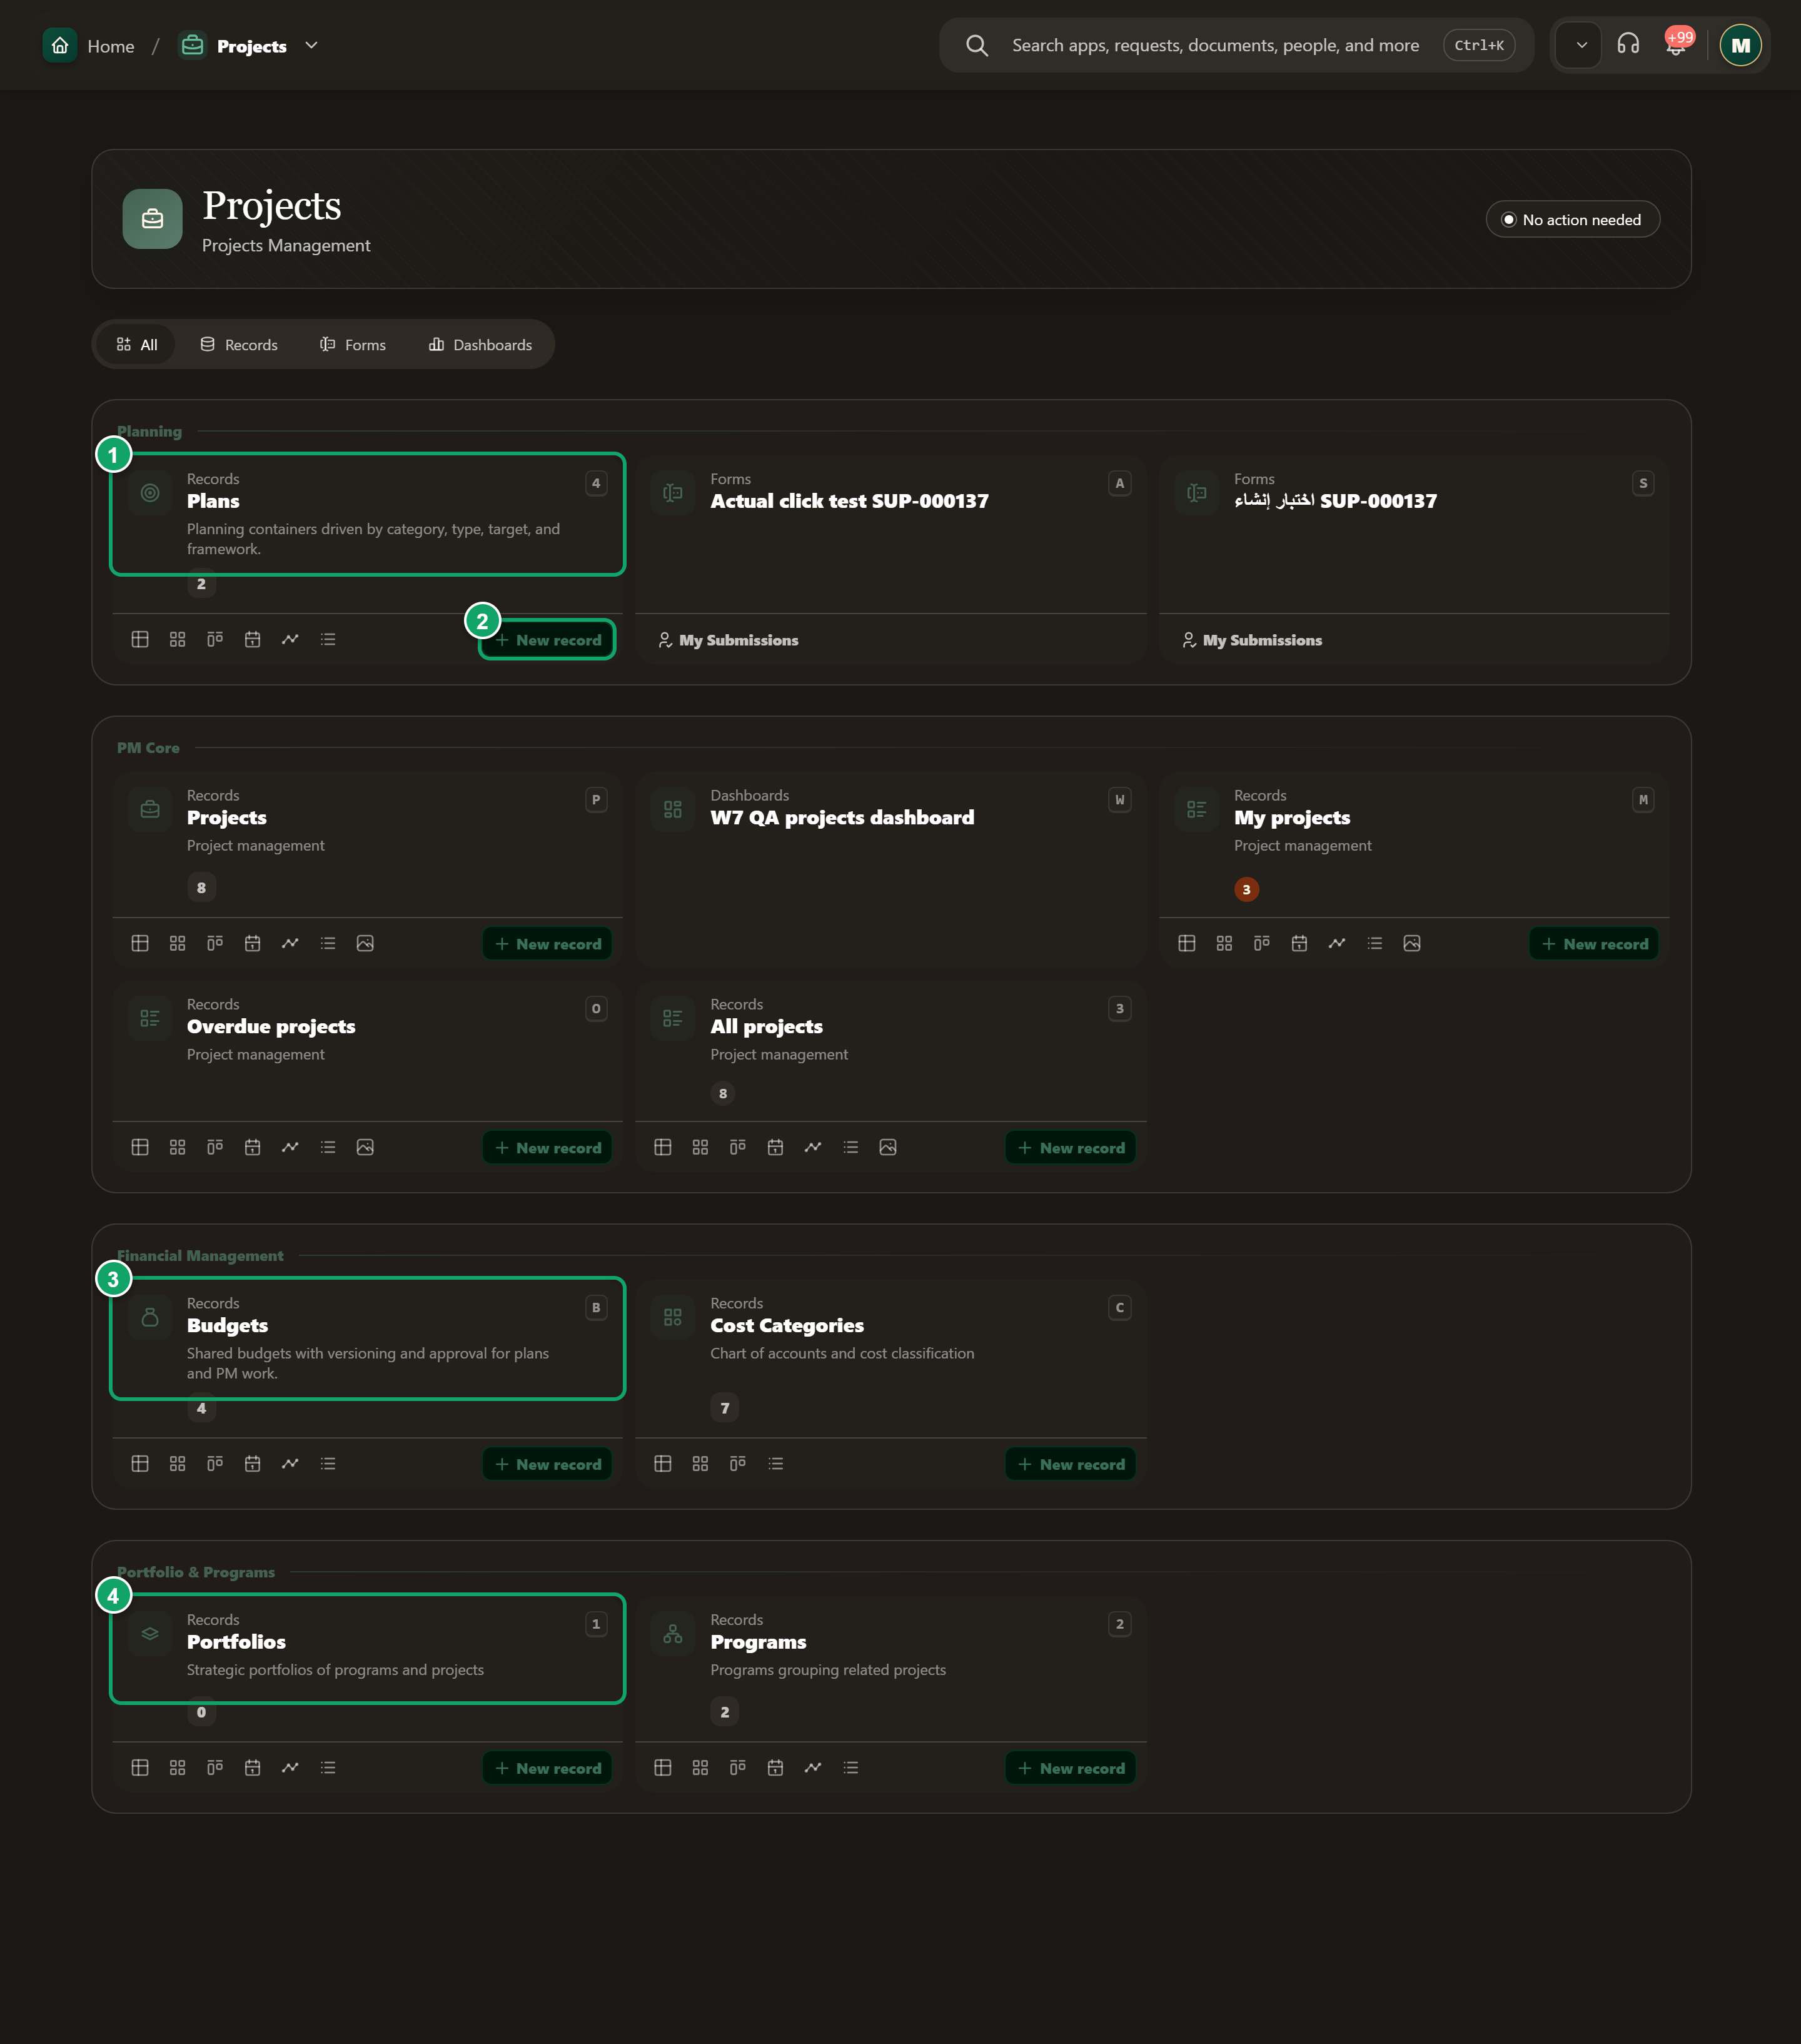
\includegraphics[width=0.95\linewidth,height=0.72\textheight,keepaspectratio]{figures/screens/ch05-directory-en.png}
\caption{Projects app entry points in test2}
\label{fig:projects-screen-directory}
\shotnote{The app cards show six main record pages and custom views available to the account. Views such as My projects show the same project records rather than a new record type; cards and counts can vary with permissions and the selected scope. Numbers on the image: ① The “Plans” card opens the plans list. ② “New record” creates a record straight from the card without opening the list. ③ The “Budgets” card in the financial section. ④ The “Portfolios” card in the portfolios and programs section.}
\end{figure}

Start with the main pages, then open the record explanation you need from the groups below. The remaining pages explain records or tools inside tabs, not separate app-menu entries. Use available list search, filters, and views to find a record; filters do not change the record itself.
\begin{table}[H]
\centering
\caption{Main pages}
\label{tab:projects-pages-foundations}
\begin{tabularx}{\linewidth}{R{4.2cm} Y}
\rcHeaderRow
\thh{Page} & \thh{What this page offers?}\\
Plans & A plan brings together the intended result, accountable target, and working period.\\
Projects & A project organizes a defined scope of work with a manager and an intended result.\\
Portfolios & A portfolio groups programs and projects that serve a common direction and helps management review priorities and funding.\\
Programs & A program coordinates related projects to achieve a shared benefit.\\
Budgets & A budget brings cost lines, funding sources, and expenditures into one record.\\
Cost Categories & Cost categories keep budget lines consistently classified, for example as travel or equipment.\\
\end{tabularx}
\end{table}
\begin{table}[H]
\centering
\caption{Objectives and results}
\label{tab:projects-pages-direction}
\begin{tabularx}{\linewidth}{R{4.2cm} Y}
\rcHeaderRow
\thh{Page} & \thh{What this page offers?}\\
Planning Themes & A strategic theme groups priorities under a clear direction.\\
Planning Objectives & An objective describes the change a plan should achieve.\\
Planning Initiatives & An initiative records proposed work that supports strategic direction.\\
OKR Cycles & An OKR cycle groups a period's objectives and the key results that measure them.\\
Key Results & A key result turns an objective into something trackable.\\
Key Result Check-ins & A key-result check-in records its state on a particular date.\\
Hoshin Items & Hoshin connects longer-term direction with annual objectives and the work needed.\\
Hoshin X-Matrix Links & Hoshin matrix links show how one item supports another.\\
Hoshin Catchball Exchanges & Catchball exchanges record proposals and responses about a Hoshin item.\\
Hoshin Countermeasures & A countermeasure records a response to a struggling Hoshin item.\\
Planning Assumptions & Assumptions record conditions the plan relies on but has not yet confirmed.\\
\end{tabularx}
\end{table}
\begin{table}[H]
\centering
\caption{Delivery and resources}
\label{tab:projects-pages-delivery}
\begin{tabularx}{\linewidth}{R{4.2cm} Y}
\rcHeaderRow
\thh{Page} & \thh{What this page offers?}\\
Planning Milestones & A milestone marks a significant result that can be checked.\\
Project Phases & A phase divides the project into ordered periods whose completion can be reviewed.\\
WBS / Work Packages & A work package breaks project scope into a portion that can be assigned and estimated.\\
Deliverables / Products & A deliverable is a result or product that can be checked at handover.\\
Requirements & A requirement states what the project must satisfy.\\
Dependencies & A dependency connects predecessor and successor work and specifies their timing relationship.\\
Planning Dependencies & A planning dependency records work that waits for another action or decision.\\
Baselines & A baseline preserves a reference for comparing an agreed plan with later results.\\
Baseline Items & A baseline item represents a saved value in a particular version.\\
Planning Resources & Plan resources record effort, cost, quantity, and capacity needs.\\
Team Roles & A team role records a member's project responsibility and allocation where used.\\
RACI Matrix & RACI identifies who performs an activity, who is accountable, who is consulted, and who is informed.\\
Resource Allocations & A resource allocation records capacity reserved for work and its utilization.\\
Stakeholders & The stakeholder register records parties involved in the project and their interest and influence.\\
Communication Plan & A communication plan defines what to share, with whom, and through which communication type.\\
\end{tabularx}
\end{table}
\begin{table}[H]
\centering
\caption{Review, quality, and risks}
\label{tab:projects-pages-governance}
\begin{tabularx}{\linewidth}{R{4.2cm} Y}
\rcHeaderRow
\thh{Page} & \thh{What this page offers?}\\
Planning Reviews & A review documents what was assessed over a defined period and the review's state.\\
Planning Approvals & An approval record captures a plan stage and its decision.\\
Planning Decisions & A decision log preserves what was decided and what needs follow-up in the plan.\\
Risk Register & A risk records a possible event that could affect the plan.\\
PM Risk Register & A project risk records a possibility affecting delivery, its impact, and the response plan.\\
Issues & An issue is an existing problem needing resolution, unlike a risk that may occur later.\\
Quality Criteria & A quality criterion defines how a result will be checked.\\
Gate Reviews & A gate review records a transition decision at a significant project point.\\
Gate Review Checks & A gate check records the result for one review criterion.\\
Change Requests & A change request records a proposed modification, its project impact, and its review workflow.\\
Meeting Decisions & A meeting decision records an agreement and its follow-up.\\
Lessons Learned & A lesson learned preserves experience useful for later work.\\
Status Reports & A status report brings together progress, risks, and notes for a defined period.\\
\end{tabularx}
\end{table}
\begin{table}[H]
\centering
\caption{Agile work}
\label{tab:projects-pages-agile}
\begin{tabularx}{\linewidth}{R{4.2cm} Y}
\rcHeaderRow
\thh{Page} & \thh{What this page offers?}\\
Sprints & A sprint divides agile work into a timebox with a goal and review.\\
Sprint Burndown Entries & A burndown entry records remaining points on a sprint day.\\
Definition of Done & The definition of done states what must be satisfied before work counts as finished.\\
\end{tabularx}
\end{table}
\begin{table}[H]
\centering
\caption{Procurement and funding}
\label{tab:projects-pages-finance}
\begin{tabularx}{\linewidth}{R{4.2cm} Y}
\rcHeaderRow
\thh{Page} & \thh{What this page offers?}\\
Procurements & A procurement record brings together a purchasing need, contract details, and financial tracking.\\
Budget Lines & A budget line details a specific cost within a budget.\\
Budget Line Periods & Budget line periods distribute amounts over time.\\
Funding Sources & A funding source records the source, pledged amount, and terms.\\
Funding Disbursements & A funding disbursement records planned and received funding from a source.\\
Expenditures & An expenditure records an actual cost against a project and budget.\\
\end{tabularx}
\end{table}
\begin{table}[H]
\centering
\caption{Measurement, evaluation, and learning}
\label{tab:projects-pages-performance}
\begin{tabularx}{\linewidth}{R{4.2cm} Y}
\rcHeaderRow
\thh{Page} & \thh{What this page offers?}\\
Performance Indicators & An indicator measures an aspect of performance using a unit, direction, and reporting frequency.\\
Time-Phased Targets & Time-phased targets distribute an intended result across periods.\\
Reporting Periods & A reporting period sets the time boundaries for measurements and reviews.\\
Planning Data Sources & A data source identifies where monitoring and evaluation information comes from.\\
Evidence Items & An evidence item preserves a reference supporting a result or finding.\\
Evaluation Questions & An evaluation question defines what you need to learn and the criterion for judging it.\\
Evaluation Findings & An evaluation finding records the review's conclusion and its implications.\\
Management Responses & A management response records what will be done about an evaluation finding or learning insight.\\
Learning Agenda Items & A learning agenda organizes questions the team needs to understand and the evidence needed.\\
Learning Insights & A learning insight records what the team learned and how it can be used.\\
Improvement Opportunities & An improvement opportunity starts with a clear problem that can be addressed.\\
Theory of Change & A theory of change connects work with expected outcomes and underlying assumptions.\\
Results Frameworks & A results framework organizes goals, outcomes, outputs, and activities.\\
Logframe Goals & A top-level goal describes the broader impact served by a results framework.\\
Logframe Outcomes & An outcome describes the expected change for those benefiting from the work.\\
Logframe Outputs & An output is a direct result that can be delivered within the framework.\\
Logframe Activities & An activity records work producing a particular output.\\
Beneficiaries & Beneficiary records describe people or groups served by the project.\\
Beneficiary Segments & Beneficiary segments break down a beneficiary record by a defined dimension.\\
\end{tabularx}
\end{table}
\begin{table}[H]
\centering
\caption{Continuity and response}
\label{tab:projects-pages-resilience}
\begin{tabularx}{\linewidth}{R{4.2cm} Y}
\rcHeaderRow
\thh{Page} & \thh{What this page offers?}\\
Planning Scenarios & A scenario describes a possible situation the plan should prepare for.\\
BIA Entries & Business impact analysis identifies an affected service and its criticality during disruption.\\
Planning Procedures & Procedures record what to do in a particular situation and how ready it is for use.\\
Planning Exercises & Exercises document a procedure or recovery test before it is needed in practice.\\
Planning Controls & A control records a preventive or oversight measure for risk or compliance.\\
Control Assessments & A control assessment records a test or effectiveness review on a specific date.\\
Planning Findings & A finding documents a gap discovered in an audit, review, or post-incident assessment.\\
Planning Incidents & An incident records a problem that has occurred and needs a response.\\
Incident Timeline Events & An incident timeline orders events by time.\\
\end{tabularx}
\end{table}
